% \documentclass[10pt]{scrartcl}
\documentclass[10pt,twocolumn]{scrartcl}

\usepackage[utf8]{inputenc}
\usepackage[T1]{fontenc}
\usepackage[ngerman]{babel}

\usepackage{amsmath}
\usepackage{amssymb}

\usepackage{graphicx}
\usepackage{tabularx}
\usepackage{authoraftertitle}

\setlength{\parindent}{0cm}
\setlength{\parskip}{3mm}
\setlength{\textheight}{23.8cm}
\setlength{\headheight}{1cm}
\setlength{\topmargin}{-10mm}

\setlength{\oddsidemargin}{0cm}
\setlength{\evensidemargin}{0cm}
\setlength{\textwidth}{16cm}
\setlength{\columnsep}{8mm}

\usepackage{multicol}
\usepackage{colortbl}
\usepackage{xcolor}
\definecolor{grau}{gray}{0.95}
\definecolor{dunkelgrau}{gray}{0.85}

\usepackage[normal]{caption}
\usepackage{lipsum}

\setlength{\parindent}{5mm}
\setlength{\parskip}{0mm}

\usepackage{float}
\restylefloat{figure}

\renewcommand{\topfraction}{0.75}
\renewcommand{\textfraction}{0.2}

%###########################################################
% die Sachen mit der Kopfzeile
\usepackage{lastpage}
\usepackage{fancyhdr}
\fancyhf{} % leere alle Felder
\fancyhead[R]{\footnotesize Phillip Schichtel: phillip.dhbw@schich.tel \\ Jonas Dann: jonas.chr.dann@gmail.com}
\fancyhead[L]{\footnotesize Ausgewählte Methoden der
Datenanalyse, \\ Modellierung und Simulation - Schattenberechnung} % Titel des Aufsatzes
\fancyfoot[C]{\footnotesize \thepage/\pageref{LastPage}}
% \fancyfoot[C]{\footnotesize \thepage}
\renewcommand{\headrulewidth}{0.4pt} % obere Trennlinie
\pagestyle{fancy}
%###########################################################

\title{Schattenberechnung im zweidimensionalen Raum}

\newcommand{\ownsection}[1]{\begin{center}\LARGE\bf#1\end{center}}

\begin{document}

\twocolumn[
\ownsection{\MyTitle}

\begin{center}
Phillip Schichtel (phillip.dhbw@schich.tel) \\
Jonas Dann (jonas.chr.dann@gmail.com) \\
Mannheim, November \the\year
\end{center}
\vspace*{5mm}
]

% \begin{multicols}{2}

\section{Abstract}

Im Folgenden werden verschiedene Methoden zur Simulation von realistischen Schatten
vorgestellt und diskutiert. Dabei werden die Verfahren "`Shadow Mapping"',
"`Ray tracing"' und "`Shadow Volumes"' theoretisch und die Implementierung
einer Abwandlung des "`Shadow Volumes"'-Verfahrens praktisch gezeigt.


\section{Einleitung \& Motivation}

Schatten gibt es überall, wo es Licht gibt. Dies gibt es zu bedenken, wenn
Gebäude oder außenbereiche geplant werden.
Desweiteren verleihen Schatten flachen Objekten eine gewisse Tiefe für das menschlische Auge.
Dies wird genutzt um in Filmen digital eingefügte Objekte realistisch aussehen zu lassen.

Aber auch in Spielen werden Schatten auf die verschiedensten Weisen verwendet. Dort werden
diese meistens auch in Echtzeit berechnet, da sich die Spielwelten in vielen Spielen sehr
häufig ändern.

Architekten nutzen Licht- und Schattensimulationen um Räume zu planen, bei denen eine passende
Ausleuchtung essentiell ist.

\subsection*{Anwendung in Spielen}

In Spielen trifft man auf viele verschiedene Anwendungen von Licht und Schatten. In den meisten
Spielen werden die Schatten genutzt, um die Spielwelt realistischer und glaubwürdiger darzustellen.
Dabei treten häufig viele verschiedene Lichtquellen in einer Szene auf, wodurch für die Berechnung der
Schatten sehr effiziente Algorithmen benötigt werden, denn eine Szene (ein Bild) muss für eine Bildrate
von 60 $\frac{\text{Bilder}}{\text{Sekunde}}$ in unter 16 Millisekunden fertig von der Grafikkarte gezeichnet sein.

Zum Zeitpunkt der Veröffentlichung dieser Arbeit ist es üblich, grobe Annäherungen zu verwenden,
wie sie etwa durch das "`Shadow Mapping"'-Verfahren berechnet werden.

Andere Spiele verwenden ähnliche Berechnungen auch für Spielelemente. So wird in dem Spiel "`Monaco"' \cite{monaco2014},
ein 2D Spiel in der Vogelperspektive, der Spieler als gerichtete Lichtquelle betrachtet um verdeckte
Elemente, also Elemente im Schatten des Blicks, auszublenden.

\subsection*{Anwendung in der Architekur}

Architekten simulieren bei neu entworfenen Gebäuden auch den Lichteinfall zu verschiedenen Tageszeiten.
Das ist besonders dann wichtig, wenn Kunden gut ausgeleuchtete Räume wollen oder auch wenn es darum geht
Sitzmöglichkeiten auf Plätzen zu planen. In ersterem will man die Schatten durch geschickte Platzierung
von Fenstern und Lampen minimieren, bei letzterem will man den Schatten zu bestimmten Tageszeiten
möglichst lange halten.

\subsection*{Anwendung in Filmen}

Viele Szenen in modernen Filmen werden heutzutage vollständig am Computer generiert. Damit diese Szenen
real aussehen, müssen auch hier wie bei den Spielen akurate Schatten berechnet werden.

\label{sec:methods}
\section{Problemstellung und Methoden}

Das Problem ist, im zweidimensionalen Raum realistische Schatten zu berechnen, die wie echte
Schatten aus den drei verschiedenen Bereichen "`Umbra"', "`Penumbra"' und "`Antumbra"' bestehen.
Also keine harten Schatten wie bei einem Punktlicht, sondern weiche Schatten und auch
Überlagerungen von Schatten.

\begin{figure}[t]
	\centering
	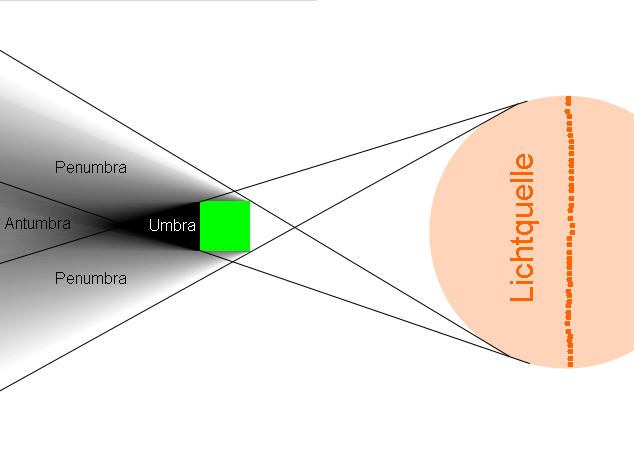
\includegraphics[width=\columnwidth]{images/umbra_penumbra_antumbra.png}
	\caption{Umbra, Penumbra \& Antumbra}
	\label{fig:umbra}
\end{figure}

\subsection{Umbra, Penumbra und Antumbra}

In der Theorie kann man bei Schatten 3 Bereiche unterscheiden (Abbildung \ref{fig:umbra}):
\begin{enumerate}
 \item \emph{Umbra}, der Kernschatten, ist der Teil des Schattens der von keinerlei Licht erreicht wird.
       Wenn es nur eine Lichtquelle gibt, dann hat jeder Schatten einen Umbra.
 \item \emph{Antumbra}, der weiche Schatten, der hinter dem Umbra entsteht. Dieser Bereich entsteht nur,
       wenn die Lichtquelle größer ist, als das Objekt, das den Schatten wirft. Der Antumbra beginnt an
       dem Punkt, an dem das Objekt die Lichtquelle nicht mehr vollständig verdecken kann und man die
       Ränder der Lichtquelle sehen kann.
 \item \emph{Penumbra}, die zwei weichen Schatten, die an den Seiten des Umbras entstehen. Diesen Bereich
       gibt es immer, wenn der Schatten nicht von einer Punktlichtquelle geworfen wird, in der realen
       Welt also immer. In diesem Bereich beginnt man die Seite der Lichtquelle zu sehen, die vorher im
       Umbra verdeckt wurde.
\end{enumerate}
Diese 3 separaten Bereiche eines Schatten sollten optisch realistisch dargestellt werden können.
Damit gilt also als Anforderung, dass Lichtquellen simuliert werden können, die eine Breite haben
und nicht einfach nur ein Punkt sind.


\subsection{Shadow Mapping}

Das "`Shadow Mapping"'-Verfahren, auch "`Projective shadowing"' genannt, berechnet eine sehr einfache,
aber dafür auch effiziente Annäherung für Schatten. Das Verfahren kann vollständig auf dem
Grafikprozessor ausgeführt werden, was nochmals zu einer Beschleunigung führt. Die Berechnung der
Szene wird dabei grob in die folgenden Schritte unterteilt:

\begin{enumerate}
 \item Als erstes wird die Szene von der Sicht des Lichts aus berechnet. Dabei wird für Punktlichter
       eine perspektivische Projektion verwendet, während für das Umgebungslicht (Sonnenlicht) eine
       orthografische Projektion verwendet wird.

       Beim berechnen der Szene in diesem Schritt werden Farben und Texturen in der Szene ignoriert,
       denn es wird nur die tiefe der Pixel benötigt um die Schatten, die in dem "`Depth Buffer"'
       (Zwischenspeicher, der Tiefeninformationen zu Pixeln hält) auf der Grafikkarte abgelegt wird.
       Für jede Lichtquelle wird dabei ein eigener Depth Buffer berechnet.
 \item Im zweiten Schritt werden die Depth Buffer auf die finale Sicht aus der ursprünglichen Kamera
       projiziert. Diese projizierten Tiefeninformationen werden dann genutzt um zu prüfen, ob ein
       Pixel im Schatten liegt oder nicht.
 \item Im letzten Schritt wird die Szene mit der ursprünglichen Kamera berechnet. Dabei wird anhand
       der vorher berechneten Depth Buffer für jeden Pixel geprüft, ob er in einem Schatten liegt.
\end{enumerate}

\subsection*{Grenzen}

Die Schatten, die mit diesem Verfahren berechnet werden, sind in der einfachsten Form harte Schatten,
die je nach Auflösung/Größe des Depth Buffer auch sehr kantig sein können (Alias-Effekt). Eine
einfache Lösung für dieses Problem ist das Weichzeichnen der Schattenkanten.

\subsection{Ray tracing}

Die Schattenberechnung durch Ray Tracing (Strahlenverfolgung) erlaubt extrem realistische Belichtungs-
und Schattenberechnungen.
Dabei sendet das Verfahren für jeden Pixel des Bildschirms einen Strahl von der Betrachterkamera aus.
Diese Strahlen werden dann über Reflektionen hinweg nachverfolgt bis sie schlussendlich in einer
Lichtquelle endet. Damit wird die exakte Belichtung berechnet, für die Schatten wird dann jeder
Kollisionspunkt betrachtet. Dort wird geprüft, ob dieser Punkt direkt von einer Lichtquelle
beschienen werden kann. Ist das nicht der Fall, dann liegt der Punkt im Schatten. Auch transparente
Objekte können mit Ray Tracing realistisch belichtet und beschattet werden.

\subsection*{Grenzen}

Mit der hohen Präzision von Ray Tracing kommt auch die entsprechend hohe Komplexität, sowohl für die
Implementierung als auch für die Laufzeit. Das Berechnen vergleichsweise einfacher Szenen kann mit
aktivem Ray Tracing mehrere Minuten dauern, was es für Schattenberechnung in Echtzeitanwendungen
unbrauchbar macht. Im Bereich der Computer Generated Imagery in der Filmproduktion findet es für die
Berechnung realistischer Schatten und in vollständig oder teilweise generierten Szenen. Hier werden
während der Produktion jedoch sehr niedrige Auflösungen (=Anzahl der Strahlen) verwendet um den
Rechenaufwand gering zu halten und schneller Ergebnisse zu erhalten.

\subsection{Shadow Volumes}

Das "`Shadow Volumes"'-Verfahren verfolgt den Ansatz, das Polygon des von einem Objekt verdeckten Bereichs
gesehen von der Lichtquelle zu berechnen. Bei diesem Ansatz agieren die Lichtquellen also ebenfalls als
Kamera, die je nach Art der Lichtquelle, die von dem Licht betroffenen Objekte in der Szene anschaut.
Dabei wird die Silhouette des momentan betrachteten Objekt gebildet und durch jeden Vertex (Eckpunkt)
ein Strahl geschossen. Der Bereich, der von den Strahlen hinter dem Objekt (gesehen von der Lichtquelle
aus) eingeschlossen wird, liegt damit im Schatten. Anschließend muss nur noch geprüft werden, ob ein zu
zeichnender Pixel in einem dieser Bereiche liegt oder nicht. Die Shadow Volumes brauchen zwar mehr
Resourcen als die einfachen Shadow Maps, sind aber dafür bedeutend präziser. In neuen Rendering-Pipelines
können die Shadow Volumes auch vollständig auf der Grafikkarte generiert werden mit Hilfe von
Geometrie-Shadern.

\subsection*{Grenzen}

Auch hier werden wie bei den Shadow Maps normalerweise nur harte Schatten berechnet, die aber ebenfalls
durch verschiedene Methoden weicher gezeichnet werden können, was in den üblichen Echtzeitanwendungen wie
Spielen ausreichend ist, auch wenn es kein realistisches Bild gibt.

\section{Durchführung}

Das entwickelte Verfahren spiegelt ein Shadow Volumes ähnliches Verfahren im zweidimensionalen
Raum wieder. Auch hier wird die Silhouette des angestrahlten Objektes berechnet und an die
Grenzen des Fensters auf dem Bildschirm projiziert. Der von dieser Projektion abgedeckte
Bereich wird dunkler eingefärbt.

Der Rasterizer wendet dann die berechnete Schattenfläche auf eine Lightmap an. Die Lightmap bildet den Beleuchtungswert jedes Pixels des Fensters ab. Der Rasterizer benötigt zwei Strahlen und ein Array von Punkten, um den Schatten auf die Lightmap zu rastern. Die zwei Strahlen bilden die Silhouette des Objektes im Raum ab. Das übergebene Array an Punkten enthält alle Eckpunkte, die auf der unbeleuchteten Seite des beleuchteten Objektes liegen. Diese werden benötigt, damit der Schatten das Rechteck nicht teilweise bis ganz überdeckt, sondern der Schatten um das Objekt herum gezeichnet werden kann. Somit kann man die Objekte in der Szene besser voneinander unterscheiden und sieht nicht ausschließlich schwarze oder graue Flächen.

Es wird vor jeder Berechnung der Schatten von einem vollkommen beleuchteten Raum ausgegangen.
Dazu wird für jeden Pixel auf dem Bildschirm der Wert 1, äquivalent zu ``von allen Lichtquellen beleuchtet'', in der Lightmap gesetzt.

\begin{figure}[t]
	\centering
	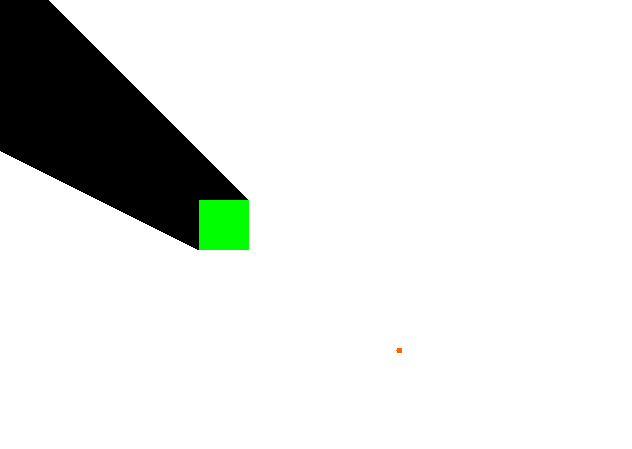
\includegraphics[width=\columnwidth]{images/durchfuehrung.png}
	\caption{einfacher Schatten}
	\label{fig:durch1}
\end{figure}

Im Folgenden wird die entwickelte Methode gezeigt um einen Schatten zu berechnen, wie er zum
Beispiel in Abbildung \ref{fig:durch1} zu sehen ist. Um diesen Schatten darstellen zu können,
werden nun zuerst die zwei Strahlen durch Eckpunkte des schattenwerfenden Objektes berechnet,
die den größten Winkel zueinander haben.

\begin{figure}[t]
	\centering
	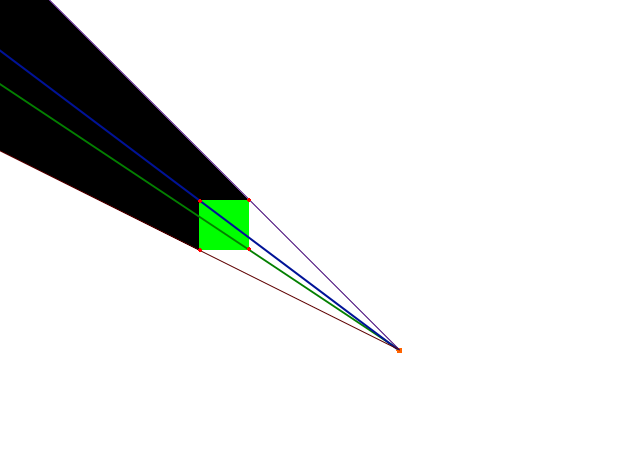
\includegraphics[width=\columnwidth]{images/durchfuehrung_1.png}
	\caption{Geraden durch Eckpunkte}
	\label{fig:durch2}
\end{figure}

Im ersten Schritt der Berechnung werden durch jeden Eckpunkt

\begin{equation}
	P = \begin{pmatrix} p_1 \\ p_2 \end{pmatrix}
\end{equation}

des schattenwerfenden Objektes und die Position der Lichtquelle

\begin{equation}
	L = \begin{pmatrix}  l_1 \\ l_2 \end{pmatrix}
\end{equation}

Geraden mit der Position des Eckpunktes als Ortsvektor und die Position der Lichtquelle subtrahiert
von der Position des Eckpunktes als Richtungsvektor
\begin{equation}
	\vec{g} = \begin{pmatrix} p_1 \\ p_2 \end{pmatrix} + r \cdot \begin{pmatrix} p_1 - l_1 \\ p_2 - l_2 \end{pmatrix}
\end{equation}
gelegt (Abbildung \ref{fig:durch2}).

\begin{figure}[t]
	\centering
	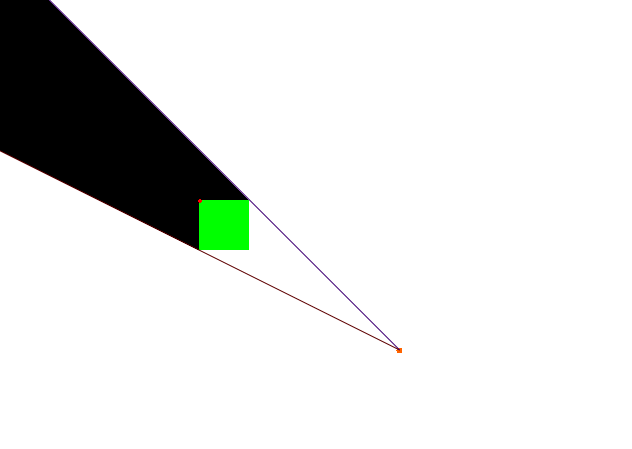
\includegraphics[width=\columnwidth]{images/durchfuehrung_4.png}
	\caption{Geraden mit größtem Winkel}
	\label{fig:durch3}
\end{figure}

Ausschlaggebend für die Silhouette des geworfenen Schatten sind die zwei Geraden, deren Winkel am
weitesten auseinander liegt (Abbildung \ref{fig:durch3}). Um diese zu bestimmen wird rekursiv jedes
Geradenpaar

\begin{equation}
  \begin{split}
	\vec{g}_1 = \vec{o}_1 + r \cdot \vec{m}_1 \\
	\vec{g}_2 = \vec{o}_2 + s \cdot \vec{m}_2
  \end{split}
\end{equation}

durch den Winkel zwischen den beiden Richtungsvektoren der Geraden

\begin{equation}
	\omega = \arccos{\left(\frac{\vec{m}_1 \cdot \vec{m}_2}{|\vec{m}_1| \cdot |\vec{m}_2|} \right)}
\end{equation}

mit dem vorherigen Geradenpaar mit dem größten Winkel zueinander verglichen und das Geradenpaar mit
dem größeren Winkel zueinander zurückgegeben.

\begin{figure}[t]
	\centering
	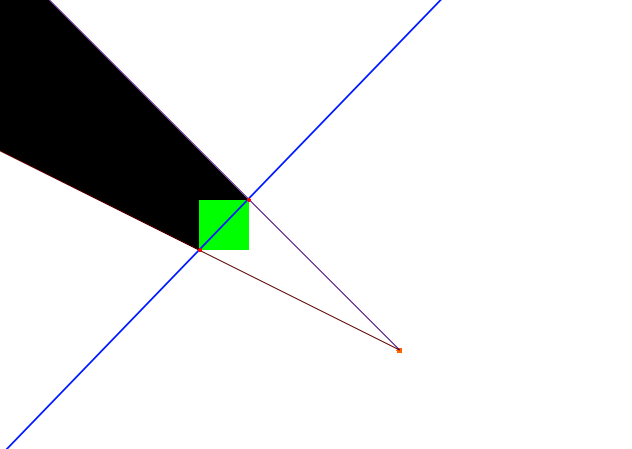
\includegraphics[width=\columnwidth]{images/durchfuehrung_2.png}
	\caption{Gerade durch Ortsvektoren}
	\label{fig:durch4}
\end{figure}

Damit später die Objekte nicht vom eigenen Schatten teilweise bis ganz überdeckt werden, werden nun die Eckpunkte des Rechtecks berechnet, welche auf der unbeleuchteten Seite des Objektes liegen. Dazu wird eine Gerade durch die Ortsvektoren der zwei vorher bestimmten Geraden erzeugt (Abbildung \ref{fig:durch4}).

\begin{equation}
	s: \vec{s} = \vec{o}_1 + t \cdot \left(\vec{o_2} - \vec{o_1}\right)
\end{equation}

\begin{figure}[t]
	\centering
	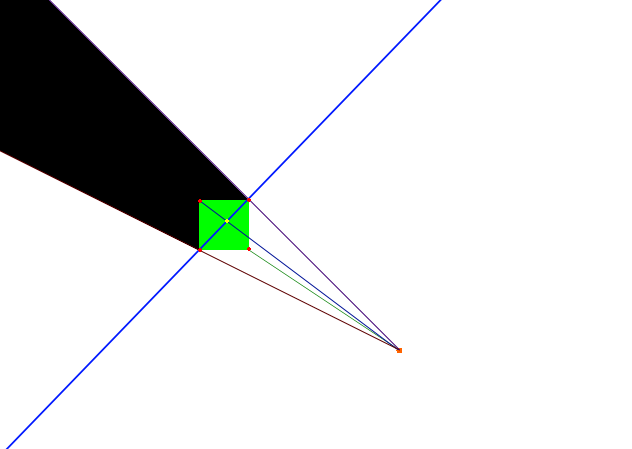
\includegraphics[width=\columnwidth]{images/durchfuehrung_3.png}
	\caption{Eckpunkte auf der dunklen Seite}
	\label{fig:durch5}
\end{figure}

Wenn ein Schnittpunkt zwischen der Geraden $s$ und der Strecke zwischen einem Eckpunkt des Rechtecks
und der Position der Lichtquelle vorhanden ist hängen wir diesen Eckpunkt an das an den Rasterizer
zu übergebende Array von Punkten an (Abbildung \ref{fig:durch5}).

Durch die Arbeitsweise des Rasterizers müssen die Schnittpunkte der zwei Silhouettenstrahlen mit den
Fenstergrenzen nicht berechnet werden. Dieses Schattenmodell, bestehend aus zwei Strahlen und einem
Array an Punkten, kann an den Rasterizer übergeben werden.

Der Rasterizer wendet dieses Konstrukt mit Hilfe des aktive Kantenlisten Algorithmus auf die
Lichtwerte der Pixel in der Szene an. Der aktive Kantenlisten Algorithmus erlaubt eine inkrementelle
Berechnung der Schnittpunkte zwischen Polygonkanten und Pixelzeilen und somit ob ein Pixel
im Polygon liegt und eingefärbt wird oder nicht. Dazu wird eine Tabelle erzeugt, die für jede Pixelzeile eine Liste an aktiven Kanten
enthält. Diese aktiven Kanten enthalten die x-Koordinate $x$ des Schnittpunktes mit der aktuellen Bildzeile, die
Differenz zwischen den x-Koordinaten der Schnittpunkte $\Delta x$ zweier vertikal benachbarter
Geraden und die Anzahl der Bildzeilen $n_y$, die von der Polygonkante noch geschnitten werden. Nun
werden die Bildzeilen inkrementell durchlaufen. Dabei werden die Kanten in einer Bildzeile nach $x$
des Schnittpunktes aufsteigend geordnet. Dann wird von $x$ der ersten Kante bis $x$ der zweiten Kante in der Liste
jedes Pixel eingefärbt. Diese beiden Kanten werden inkrementiert und die nächsten beiden Kanten werden
betrachtet, bis keine Kanten mehr in der Bildzeile übrig sind. Dann wird die nächste Bildzeile
nach dem selben Schema behandelt. Eine Kanten wird inkrementiert indem die Kante in die nächsthöhere Bildzeile verschoben
wird, $x$ auf $x + \Delta x$ gesetzt und $n_y$ dekrementiert wird.


Durch die Beschaffenheit dieses Algorithmus wird für den übergebenen Schatten in vielen Fällen nicht das komplette Polygon ausgerechnet.

\section{Ergebnisse}

\begin{figure}[t]
	\centering
	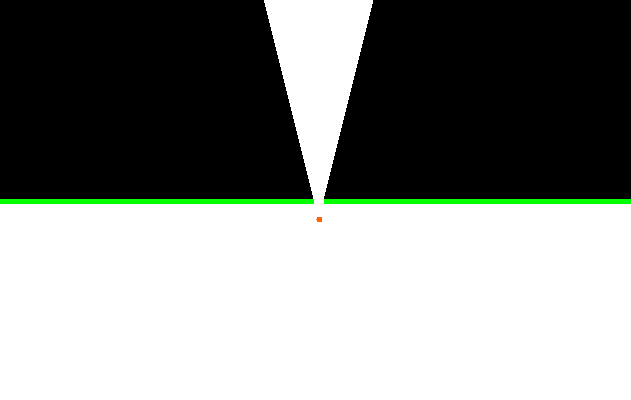
\includegraphics[width=\columnwidth]{images/ergebnis_3.png}
	\caption{Harter Schatten}
	\label{fig:ergeb4}
\end{figure}

Das Ziel der Berechnung von Schatten ist die Darstellung möglichst real wirkender Beleuchtung. In
der realen Welt werfen Lichter, wenn sie auf undurchsichtige Objekte treffen für gewöhnlich, keine
harten Schatten, wie in Abbildung \ref{fig:ergeb4}.

\begin{figure}[t]
	\centering
	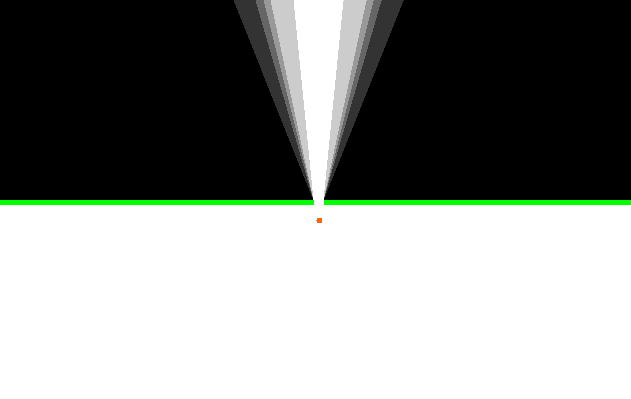
\includegraphics[width=\columnwidth]{images/ergebnis_2.png}
	\caption{Annäherung weicher Schatten}
	\label{fig:ergeb3}
\end{figure}

Weichere Schatten, wie in Abbildung \ref{fig:ergeb3}, können durch das Darstellen einer Lichtquelle
als Menge von leicht versetzten Lichtquellen erreicht werden.

\begin{figure}[t]
	\centering
	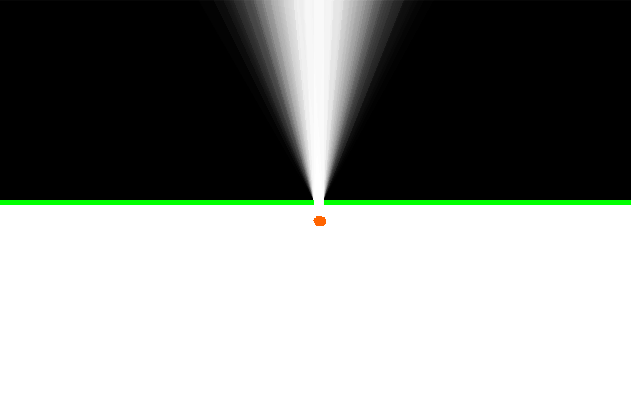
\includegraphics[width=\columnwidth]{images/ergebnis.png}
	\caption{Weiche Schatten}
	\label{fig:ergeb2}
\end{figure}

Durch eine weitere Erhöhung der Zahl, der Lichtquellen, kann eine noch realistischere Annäherung
vorgenommen werden. Umso mehr Lichtquellen bei der Annäherung verwendet werden, desto glatter ist
der Verlauf zwischen Schatten und Licht.

\begin{figure}[t]
	\centering
	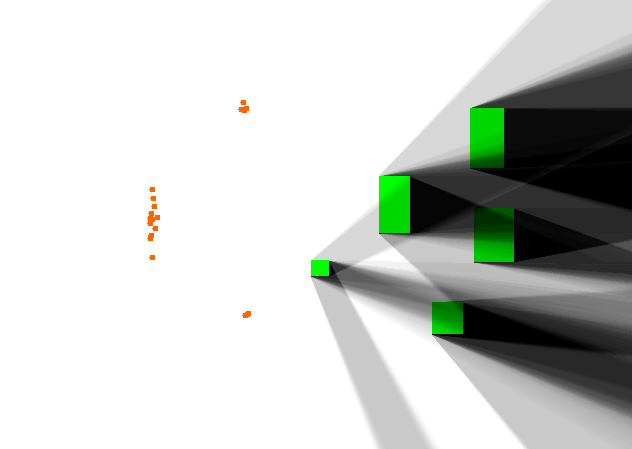
\includegraphics[width=\columnwidth]{images/ergebnis_4.png}
	\caption{Komplexe Szene}
	\label{fig:ergeb1}
\end{figure}

Abbildung \ref{fig:ergeb1} zeigt eine Szene mit vielen Lichtquellen und schattenwerfenden Objekten.
Zum einen wird hier ein weiteres Mal der an \ref{fig:ergeb2} gezeigte Effekt sichtbar. Schatten
sind nah am Objekt noch sehr hart und werden mit wachsendem Abstand zum schattenwerfenden Objekt
weicher. Zum anderen sieht man die Überlagerung von Schatten mehrerer Lichtquellen. Je nachdem wie
viele Lichtquellen auf ein Pixel scheinen wird dieses mehr oder weniger hell eingefärbt. Durch die
Annäherung großer flächenartiger Lichtquellen durch viel kleine Punktlichter entstehen Umbra,
Penumbra und Antumbra.

\section{Diskussion}

Der entwickelte Ansatz deckt sehr viel der gegebenen Problemstellung ab. Schatten werden im zweidimensionalen gezeichent
und weisen weich verlaufende Kanten auf. Verschiedene Objekte und Lichter können in die Szene gesetzt
werden. Für viele Anwendungen zum Beispiel im Videospielebereich reicht dieser Ansatz aus. Jedoch
muss die Lösung spätestens bei der Übersetzung in den dreidimensionalen Raum erweitert werden.

\subsection{Grenzen des gewählten Ansatz}

Größter Kritikpunkt an dem gezeigten Verfahren ist die Beschränkung auf den zweidimensionalen Raum.
Für einige Spiele- und Userinterfaceprojekte würden diese Schatten ausreichen, jedoch wird heutzutage in Filmen und großen Videospieleproduktionen
viel Wert auf möglichst realitätsnahe computergenerierte Grafiken
gelegt. Dafür werden die in Kapitel \ref{sec:methods} beschriebenen Methoden benötigt.

Die entwickelte Anwendung ist auf Rechtecke im Raum beschränkt, die an den Koordinatenachsen
ausgerichtet sind. Jedoch kann diese signifikante Einschränkung behoben werden, da der
momentane Programmcode mit leichten Modifikationen auch andere Formen unterstützen kann.

Die Performance der Berechnungen ist ein weiterer Kritikpunkt der entwickelten Methode. Die Laufzeit
steigt zwar in Abhängigkeit der Lichter als auch der Objekte auf dem Bildschirm linear an, jedoch
ist Berechnungsdauer bei mehreren hundert Lichtern und Objekten im Verhältnis zur Komplexität des
Algorithmus zu hoch um diese Methode mit komplexen Szenen in Echtzeitanwendungen einsetzen zu können.

Der entwickelte Algorithmus ist durch die genannten Einschränkungen am Besten in zweidimensionalen
Videospielen einsetzbar. Dort können solche Berechnungen für das Sichtfeld des Spielers oder wie in
der entwickelten Anwendung zur Schattenberechnung eingesetzt werden. Hier kann es auch interessant
sein die Schattenberechnung zu erweitern und Licht komplexer darzustellen. Der erste Schritt zur
Erweiterung in diese Richtung wäre die Einführung von farbigen Lichtern. Somit könnten farbliche
Überlagerungen zur Erzeugung interessanter Effekte genutzt werden.

Weiterhin könnten die schon implementierten Materialien, welche bis jetzt nur zur Speicherung der
Farbe der Objekte in der Szene genutzt werden, mit Transparenz erweitert werden. Verschiedene
Materialien brechen Licht in unterschiedlichen Weisen.

Die Schattenberechnungsmethode bietet Möglichkeiten Lichtstreuung und -reflektion zu
implementieren. Auch hierzu müssten die Materialien erweitert werden, jedoch könnten dann realistischere und grafisch ansprechendere Szenen dargestellt werden.

Eine Problematik die auch in den heutigen sehr realistischen Schattenberechnungsalgorithmen bleibt ist die Lichtbeugung an Objektkanten. Diesen Effekt nähert der entwickelte Algorithmus mit der Nutzung vieler Punktlichtquellen anstelle einer flächenartigen Lichtquelle an. Darüber hinaus hat der Effekt in den meisten praktischen Anwendungen keine Bedeutung, da er nur sehr schwach und für das menschliche Auge nicht sichtbar ist.

\subsection{Alternative Ansätze}

Bei komplexen Szenen stößt die hier gezeigte Implementierung des Algorithmus durch verschiedene Faktoren an ihre Grenzen. Jedoch kann dieses Problem
gelöst werden. Zum Einen gibt es die Möglichkeit Schatten komplett oder teilweise statisch zu berechnen.
Dies ist möglich, wenn sich die Lichtquellen oder Objekte im Raum nicht oder nur teilweise bewegen. Das
ist zum Beispiel der Fall wenn sich ein Objekt innerhalb des beschatteten Bereich bewegt ohne eine der
Schattenkanten zu berühren.
In jedem Fall können komplett statische Lightmaps, welche zu jedem Pixel in der Szene einen
Beleuchtungswert speichern, mit dynamischen Lightmaps verrechnet werden um Rechenaufwand zu sparen. Weiterhin könnte den Rasterizer der Grafikkarte genutzt werden um Polygone auf den Bildschirm zu zeichnen. Dieser ist trotz des momentan verwendeten sehr effizienten aktiven Kantenlisten Algorithmus viel schneller, da er die Beschleunigung durch die Grafikkarte nutzt. Weitere Optimierungen sind möglich.

\subsubsection*{Ray casting}

Ein alternativer Ansatz wäre "`Ray casting"' gewesen, eine einfache Form des Ray tracing. Im zweidimensionalen
Raum werden dabei eine bestimmte festdefinierte Anzahl an Strahlen in alle Richtungen von jeder Lichtquelle
aus geschossen. Dabei laufen diese Strahlen bis zum ersten Punkt an dem sie mit einem Objekt kollidieren
oder bis zum Rand des Bildes beziehungsweise des Simulationsbereichs.

Im Vergleich zu dem von gewählten Verfahren müssten hier bedeutend mehr Strahlen berechnet werden um die
selben präzisen Schatten zu erhalten. Je nach Distanz, die die Strahlen zurücklegen müssen, muss die Anzahl
der Strahlen beim Ray casting erhöht werden um weiterhin genaue Schatten liefern zu können, denn die Strahlen
laufen gemäß der Kreisumfangsformal mit steigendem Radius auseinander. Auf das implementierte Verfahren hat
die Distanz zur Lichtquelle keinen Einfluss, denn es werden direkt die Ecken der Objekte betrachtet.

\subsection{Abdeckung der Problematik}

Eine Schattenberechnung im zweidimensionalen Raum wurde implementiert. Diese Schatten umfassen je nach Konstellation der Objekte und Lichter Umbra, Penumbra
und Antumbra. Auch harte Schatten werden durch die Annäherung
großer flächenartiger Lichtquellen durch viele kleine Punktlichter auf elegante Art und Weise vermieden und realitätsnah
dargestellt. Für viele Videospiele im zweidimensionalen Raum reicht diese Art von Schattenberechnung aus,
jedoch bleibt Erweiterungsspielraum. Weitere Implementierungen von farbigen Lichtern und die Unterstützung
von komplexeren Materialien für die Objekte im Raum sind für die Zukunft denkbar und mit dem entwickelten Code möglich.



\begin{thebibliography}{99}
\bibitem{monaco2014}http://www.monacoismine.com/
\bibitem{Goos1947}F.Goos und H.Hänchen: {\it Ein neuer fundamentaler Versuch zur Totalreflektion}, 1947; Annalen der Physik 436, S. 333-346
\bibitem{Einstein1905}A.Einstein {\it Zur Elektrodynamik bewegter Körper}, 1905; Annalen der Physik und Chemie 17, S. 891-921
\bibitem{Gerhards2008}H.Gerhards: {\it Ground Penetrating Radar as a Quantative Tool with Applications in Soil Hydrology}, Heidelberg 2008; Dissertaton,
\bibitem{Wittgenstein1922}L.Wittgenstein: {\it Tractatus Logico-Philo\-so\-phi\-cus}, London 1922; Kegan Paul, Trench, Trubner \& Co., Ltd.
\end{thebibliography}

\end{document}
